\begin{frame}
	\myheading{Module 8.9 : Early stopping}
\end{frame}

\begin{frame}
	\vspace{4em}
	\begin{overlayarea}{\textwidth}{\textheight}
		\begin{block}{Other forms of regularization}
			\begin{itemize}
				\item $l_2$ regularization
				\item Dataset augmentation
				\item Parameter Sharing and tying
				\item Adding Noise to the inputs
				\item Adding Noise to the outputs 
				\item \textcolor<2->{red}{Early stopping}
				\item Ensemble methods
				\item Dropout
			\end{itemize}
		\end{block}
	\end{overlayarea}
\end{frame}


\begin{frame}
	\begin{columns}
		\column{0.5\textwidth}
		\begin{overlayarea}{\textwidth}{\textheight}
			\only<1->{
				\begin{figure}
					\input{modules/Module9/tikz_images/tikz1}
				\end{figure}
			}
		\end{overlayarea}
		\column{0.5\textwidth}
		\begin{overlayarea}{\textwidth}{\textheight}
			\begin{itemize}
				\justifying
				\item<1-> Track the validation error
				\item<2-> Have a patience parameter $p$
				\item <3-> If you are at step $k$ and there was no improvement in validation error in the previous $p$ steps then stop training and return the model stored at step $k-p$
				\item <4-> Basically, stop the training early before it drives the training error to $0$ and blows up the validation error
			\end{itemize}
		\end{overlayarea}
	\end{columns}
\end{frame}

\begin{frame}
	\begin{columns}
		\column{0.5\textwidth}
		\begin{overlayarea}{\textwidth}{\textheight}
			%Figure :
			\only<1->{
				\begin{figure}
					
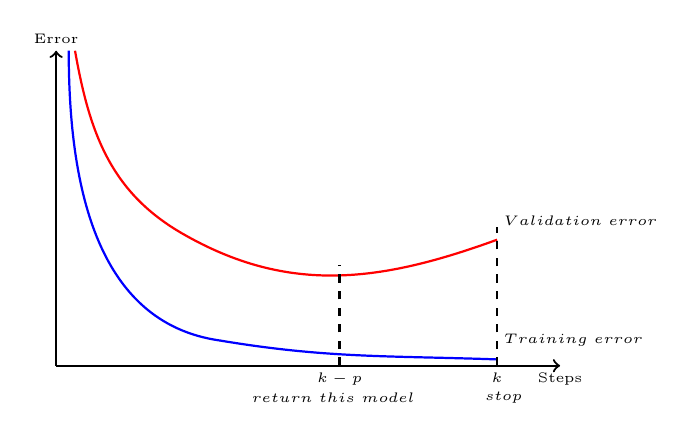
\begin{tikzpicture}[scale=0.8]
	\tiny
	\draw[thick,->] (0,0) -- (8,0) node [below] {Steps};
	\draw[thick,->] (0,0) -- (0,5) node [above] {Error};
	\draw[thick,blue] (0.2,5) to [out=270,in=172] (2.6,0.4);
	\draw[thick,blue] (2.6,0.4) to [out=350.5,in=178] (7,0.1);
	\node [right] at (7,0.4) {$Training$ $error$};
	\draw[thick,red] (0.3,5) to [out=280,in=150] (2,2.1);
	\draw[thick,red] (2,2.1) to [out=330,in=200] (7,2);
	%\draw[snake=sn[red]e]  (2,2.1) -- (7,2);
	\node [right] at (7,2.3) {$Validation$ $error$};
	\draw[thick,dashed] (4.5,0) node[below]{$k-p$}--(4.5,1.6);
	\draw[thick,dashed] (7,0) node[below]{$k$}--(7,2.2);
	\node [right] at (6.7,-0.5) {$stop$};
	\node [right] at (3,-0.5) {$return$ $this$ $model$};
	%\draw (0,2) to [out=340,in=200] (7,1.8);
	%\node [right] at (7,1.8) {$AVC$};
	%\draw (0,2) to [out=315,in=240] (7,5);
	%\node [right] at (7,5) {$MC$};
\end{tikzpicture}
				\end{figure}
			}
		\end{overlayarea}
				
		\column{0.5\textwidth}
		\begin{overlayarea}{\textwidth}{\textheight}
			\begin{itemize}
				\justifying
				\item<1-> Very effective and the mostly widely used form of regularization
				\item<2-> Can be used even with other regularizers (such as $l_2$)
				\item <3-> How does it act as a regularizer ?
				\item <4-> We will first see an intuitive explanation and then a mathematical analysis
			\end{itemize}
		\end{overlayarea}
	\end{columns}
\end{frame}

\begin{frame}
	\begin{columns}
		\column{0.5\textwidth}
		\begin{overlayarea}{\textwidth}{\textheight}
			\only<1->{
				\begin{figure}
					\input{modules/Module9/tikz_images/tikz4}
				\end{figure}
			}
		\end{overlayarea}
				
		\column{0.5\textwidth}
		\begin{overlayarea}{\textwidth}{\textheight}
			\begin{itemize}
				\justifying
				\item<1-> Recall that the update rule in SGD is 
				\begin{align*}
					\onslide<2->{w_{t+1} & =w_{t}-\eta \nabla w_{t}               \\}
					\onslide<3->{             & =w_{0}-\eta \sum_{i=1}^{t}\nabla w_{i}}
				\end{align*}
				\item <4-> Let $\tau$ be the maximum value of $\nabla w_i$ then
						\begin{align*}
							\onslide<5->{ & |w_{t+1} - w_{0}| \leq \eta t |\tau|} 
						\end{align*}
				\item <6-> Thus, $t$ controls how far $w_t$ can go from the initial $w_0$
				\item<7->In other words it controls the space of exploration
			\end{itemize}
		\end{overlayarea}
	\end{columns}
\end{frame}

\begin{frame}
	\begin{block}{}
		We will now see a mathematical analysis of this
	\end{block}
\end{frame}

\begin{frame}
	\begin{columns}
		\column{1.0\textwidth}
		\begin{overlayarea}{\textwidth}{\textheight}
						
			\begin{itemize}
				\justifying
								
				\item<1-> Recall that the Taylor series approximation for $\mathscr{L}(w)$ is
			\end{itemize}
			\begin{align*}
				\onslide<2-> {\mathscr{L}(w)        & =\mathscr{L}(w^{*})+(w -w^{*})^{T}\nabla \mathscr{L}(w^{*})+\frac{1}{2}(w-w^{*})^{T}H(w-w^{*})}                                   \\
				\onslide<3-> {                 & =\mathscr{L}(w^{*})+\frac{1}{2}(w-w^{*})^{T}H(w-w^{*}) \hspace{1.5cm} [\ w^{*}\  is\ optimal\ so\ \nabla \mathscr{L}(w^{*})\ is\ 0\ ]} \\
				\onslide<4->{\nabla(\mathscr{L}(w)) & =H(w-w^{*})} 
				%\onslide<3>{\Delta(\mathscr{L}(w))&=H(w-w^{*})}
			\end{align*}

			\onslide<5->Now the SGD update rule is:
			\begin{align*}
				\onslide<6->{w_t & =w_{t-1}-\eta \nabla \mathscr{L}(w_{t-1} )    \\}
				\onslide<7->{         & =w_{t-1}-\eta H(w_{t-1}-w^{*}) \\}
				\onslide<8->{         & =(I-\eta H)w_{t-1}+\eta H w^{*}     \\}
			\end{align*}
		\end{overlayarea}
	\end{columns}
	%\end{itemize}
\end{frame}

\begin{frame}
	%\column{0.70\textwidth}
	%\begin{overlayarea}{\textwidth}{\textheight}
	\begin{align*}
		\onslide<1->w_t=(I-\eta H)w_{t-1}+\eta H w^{*} 
	\end{align*}
	\begin{itemize}
		\justifying
		\item<2-> Using EVD of $H$ as $H=Q \Lambda Q^{T}$, we get:
		\begin{align*}
			w_t=(I-\eta Q \Lambda Q^{T} )w_{t-1}+\eta Q \Lambda Q^{T} w^{*} 
		\end{align*}
		\item<3-> If we start with $w_{0}=0$ then we can show that (See Appendix)
		\begin{align*}
			w_t=Q[I-(I-\varepsilon \Lambda)^{t}]Q^{T}w^{*} 
		\end{align*}
		\item<4-> Compare this with the expression we had for optimum $\tilde{W}$ with $L_2$ regularization
		\begin{align*}
			\tilde{w}=Q[I-(\Lambda+ \alpha I)^{-1} \alpha]Q^{T}w^{*} 
		\end{align*}
		\item<5-> We observe that $w_t=\tilde{w}$, if we choose $
		\varepsilon$,$t$ and $\alpha$ such that 
		\begin{align*}
			(I-\varepsilon \Lambda)^{t}=(\Lambda+ \alpha I)^{-1} \alpha 
		\end{align*}
		%\end{overlayarea}
		%\end{columns}
	\end{itemize}
\end{frame}

\begin{frame}
	\begin{block}{Things to be remember}
		\begin{itemize}
			\justifying
			\item<1-> Early stopping only allows $t$ updates to the parameters.
			\item<2-> If a parameter $w$ corresponds to a dimension which is important for the loss $\mathscr{L}(\theta)$ then $\frac{\partial \mathscr{L}(\theta)}{\partial w}$ will be large
			\item<4-> However if a parameter is not important ($\frac{\partial \mathscr{L}(\theta)}{\partial w}$ is small) then its updates will be small and the parameter will not be able to grow large in $`t'$ steps
			\item<5-> Early stopping will thus effectively shrink the parameters corresponding to less important directions (same as weight decay).
		\end{itemize}
	\end{block}
\end{frame}
